\documentclass[a4paper, openany]{memoir}

\usepackage[utf8]{inputenc}
\usepackage[T1]{fontenc} 
\usepackage[english]{babel}
\usepackage{fancyhdr}
\usepackage{float}
\usepackage{amsmath, amsthm, amssymb}
\usepackage{enumitem}
\usepackage[bookmarksopen=true,bookmarksopenlevel=2]{hyperref}
\usepackage{tikz}
\usepackage{pgfplots}
\usepackage{indentfirst}
\usepackage{pgfplots}
\usepackage{listings}
\usepackage{xcolor}

\pagestyle{fancy}
\fancyhf{}
\fancyhead[LE]{\leftmark}
\fancyhead[RO]{\rightmark}
\fancyhead[RE, LO]{Database Systems}
\fancyfoot[LE, RO]{\thepage}
\fancyfoot[RE, LO]{Pete Gautam}

\renewcommand{\headrulewidth}{1.5pt}

\definecolor{codegreen}{rgb}{0,0.6,0}
\definecolor{codegray}{rgb}{0.5,0.5,0.5}
\definecolor{codepurple}{rgb}{0.58,0,0.82}
\definecolor{backcolour}{rgb}{0.95,0.95,0.92}

\newcommand{\bnode}[3]{
    \draw (0+#1, 0+#2) -- (4.25+#1, 0+#2)
        -- (4.25+#1, 0.5+#2) 
        -- (0+#1, 0.5+#2)
        -- cycle;
    \foreach \i in {0.75, 1.75, 2.5, 3.5} {
        \draw (\i+#1, 0+#2) -- (\i+#1, 0.5+#2);
    }
    \foreach \i in {0, 1.75, 3.5} {
        \draw[fill=black] (\i+0.75/2+#1, 0.25+#2) circle (2pt);
    }
    \foreach \i in {0.75, 2.5} {
        \filldraw[red] (\i+0.75+#1, 0.25+#2) circle (2pt);
    }
    \foreach \x[count=\i] in {#3} {
        \node at (1.75*\i+#1-0.675, 0.25+#2) {\texttt{\x}};
    }
}

\newcommand{\bplusinternalnodesng}[3]{
    \draw (0+#1, 0+#2) -- (5*0.75+#1, 0+#2)
    -- (5*0.75+#1, 0.5+#2) 
    -- (0+#1, 0.5+#2)
    -- cycle;
    \foreach \i in {1, 2, 3, 4} {
        \draw (\i*0.75+#1, 0+#2) -- (\i*0.75+#1, 0.5+#2);
    }
    \foreach \i in {0, 2} {
        \draw[fill=black] (\i*0.75+0.75/2+#1, 0.25+#2) circle (2pt);
    }
    \foreach \x[count=\i] in {#3} {
        \node at (\i*0.75*2-0.75+0.75/2+#1, 0.25+#2) {\texttt{\x}};
    }
}

\newcommand{\bplusinternalnodedbl}[3]{
    \draw (0+#1, 0+#2) -- (5*0.75+#1, 0+#2)
    -- (5*0.75+#1, 0.5+#2) 
    -- (0+#1, 0.5+#2)
    -- cycle;
    \foreach \i in {1, 2, 3, 4} {
        \draw (\i*0.75+#1, 0+#2) -- (\i*0.75+#1, 0.5+#2);
    }
    \foreach \i in {0, 2, 4} {
        \draw[fill=black] (\i*0.75+0.75/2+#1, 0.25+#2) circle (2pt);
    }
    \foreach \x[count=\i] in {#3} {
        \node at (\i*0.75*2-0.75+0.75/2+#1, 0.25+#2) {\texttt{\x}};
    }
}

\newcommand{\bplusleafnodedbl}[3]{
    \draw (0+#1, 0+#2) -- (2+#1, 0+#2)
    -- (2+#1, 0.5+#2)
    -- (0+#1, 0.5+#2)
    -- cycle;

    \draw (1+#1, 0+#2) -- (1+#1, 0.5+#2);

    \foreach \x[count=\i] in {#3} {
        \filldraw[red] (\i-0.25+#1, 0.25+#2) circle (2pt);
        \node at (\i-0.75+#1, 0.25+#2) {\texttt{\x}};
    }
}

\newcommand{\bplusleafnodesng}[3]{
    \draw (0+#1, 0+#2) -- (1+#1, 0+#2)
    -- (1+#1, 0.5+#2)
    -- (0+#1, 0.5+#2)
    -- cycle;

    \filldraw[red] (0.75+#1, 0.25+#2) circle (2pt);
    \node at (0.25+#1, 0.25+#2) {\texttt{#3}};
}

\lstdefinestyle{thestyle}{
    backgroundcolor=\color{backcolour},
    basicstyle=\ttfamily\footnotesize,
    keywordstyle=\color{red!80}\bfseries,
    ndkeywordstyle=\color{blue!80}\bfseries,
    identifierstyle=\color{black},
    commentstyle=\color{codegreen},
    stringstyle=\color{codepurple},
    breakatwhitespace=false,
    breaklines=true,
    captionpos=b,
    keepspaces=true,
    % numberstyle=\tiny\color{codegray},
    % numbers=left,
    % numbersep=2pt,
    showspaces=false,
    showstringspaces=false,
    showtabs=false,          
    tabsize=2
}

\lstset{style=thestyle}
\chapterstyle{thatcher}
\setcounter{chapter}{2}
\pgfplotsset{compat=newest}

\begin{document}
\chapter{Design and Query}
\section{Physical Design}
There is a 3-level storage hierarchy- primary storage, main memory such as RAM and cache; secondary storage, such as hard-drive disks (HDD) and solid-state disks (SSD); and tertiary storage, such as optical drives. As we go down the storage hierarchy, the storage capacity increases, but access speed decreases significantly, and the price decreases.

The fundamental challenge is that a database is too large to fit in the main memory. So, we have to store them in secondary storage (i.e. hard disks). This has the following consequences:
\begin{itemize}
    \item Since the hard disk is not CPU-accessible, we need to first load the data into main memory from the disk, and then process it in the main memory.
    \item The speed of data access becomes low- data access from HDD takes 30ms, while it only takes about 30ns in RAM.
\end{itemize}
So, the main bottleneck is transferring data from the disk to main memory. We will organise data on disks in such a way that minimises this latency.

Our first challenge is therefore to organise tuples on the disk to minimise I/O access cost. We will first consider how data is represented. A tuple is represented as a record- a sequence of binary digits. Records are grouped together into blocks. A file is composed of many blocks. This is illustrated below.
\begin{figure}[H]
    \centering
    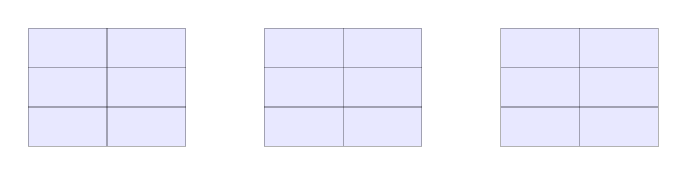
\begin{tikzpicture}
        \foreach \x in {0, 1, 2} {
            \draw[fill=blue!30, opacity=0.3] (\x*3, 0) -- (\x*3, 1.5)
                -- (\x*3+2, 1.5)
                -- (\x*3+2, 0)
                -- cycle;
            
            \draw[fill=blue!30, opacity=0.3] (\x*3+1, 0) -- (\x*3+1, 1.5);
            \foreach \y in {0.5, 1} {
                \draw[fill=blue!30, opacity=0.3] (\x*3, \y) -- (\x*3+2, \y);
            }
        }
    \end{tikzpicture}
    \caption{A file stored in blocks}
\end{figure}

Records can be of fixed or variable length. This depends on whether the attributes have a fixed size (in bytes), or whether the size of the attributes can vary. We will assume that the attributes have fixed size. 

For example, assume that we have the following attributes in a tuple:
\begin{itemize}
    \item \texttt{Name}, which takes 30 bytes;
    \item \texttt{SSN}, which takes 10 bytes;
    \item \texttt{Salary}, which takes 4 bytes;
    \item \texttt{Job\_Code}, which takes 4 bytes;
    \item \texttt{Department}, which takes 20 bytes; and
    \item \texttt{Hire\_Date}, which takes 6 bytes.
\end{itemize}
Then, a tuple takes
\[30 + 10 + 4 + 4 + 20 + 6 = 74\]
bytes.

A block is of fixed length. It is somewhere between 512 bytes and 4096 bytes typically. If we have a record of $R$ bytes and a block of $B$ bytes. The blocking factor (\textit{bfr}) is the number of records that can be stored in a block. It is given by
\[\textit{bfr} = \operatorname{floor}(B/R).\]
For example, if $\textit{bfr} = 100$, then we can store up to 100 records in a single block. We must have at least one record per block, so we require $B \geq R$.

Another challenge is how we allocate the blocks of files on the disk. We can use linked allocation. Here, each block $i$ has a pointer to the physical address to the logically next block $i+1$ anywhere on the disk. So, it is essentially a linked list of blocks. This is illustrated below.
\begin{figure}[H]
    \centering
    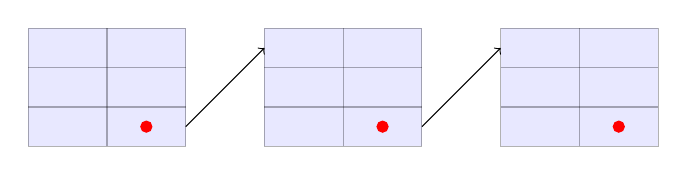
\begin{tikzpicture}
        \foreach \x in {0, 1, 2} {
            \draw[fill=blue!30, opacity=0.3] (\x*3, 0) -- (\x*3, 1.5)
                -- (\x*3+2, 1.5)
                -- (\x*3+2, 0)
                -- cycle;
            
            \draw[fill=blue!30, opacity=0.3] (\x*3+1, 0) -- (\x*3+1, 1.5);
            \foreach \y in {0.5, 1} {
                \draw[fill=blue!30, opacity=0.3] (\x*3, \y) -- (\x*3+2, \y);
            }
            \filldraw[red] (\x*3+1.5, 0.25) circle (2pt);
        }
        
        \draw[->] (2, 0.25) -- (3, 1.25);
        \draw[->] (5, 0.25) -- (6, 1.25);
    \end{tikzpicture}
    \caption{A file as a linked list of blocks}
\end{figure}

Now, assume we have the relation \texttt{Employee} with $r = 1103$ tuples, each one corresponding to a fixed-length record. Moreover, each record has the following fields:
\begin{itemize}
    \item \texttt{Name} (30 bytes),
    \item \texttt{SSN} (10 bytes), and
    \item \texttt{ADDRESS} (60 bytes).
\end{itemize}
So, each tuple takes
\[30 + 10 + 60 = 100\]
bytes. Therefore, the tuple size $R = 100$ bytes. Then, if the block size $B = 512$, we have the blocking factor
\[\textit{bfr} = \operatorname{floor}(B/R) = 5.\]
This means that we can store at most 5 tuples per a block. So, to store all $r = 1103$ tuples, we need
\[b = \operatorname{ceil}(r/\textit{bfr}) = 221\]
blocks to store all the records.

Our next challenge is to distribute records within blocks to minimise I/O cost. For this, we will consider 3 representations of data:
\begin{itemize}
    \item heap (or unordered) file, where we add a new record to the end of the file.
    \item ordered (or sequential) file, where we keep the records physically sorted with respect to some ordering field.
    \item hash file, which makes use of a hash function to each record, and uses this as the physical block address.
\end{itemize}
If we use ordered file, then we need to decide on the ordering field. Similarly, if we use hash file, then we need to choose the hash field. This should be done in a way that minimises the I/O cost.

We define I/O access cost as the cost for:
\begin{itemize}
    \item retrieving a whole block from the disk to memory to search for a record with respect to some searching field(s) (the search cost); and
    \item inserting, deleting or updating a record by transferring the whole block from memory to disk (the update cost).
\end{itemize}
The cost function is the expected number of block accesses (read or write) to search, insert, delete or update a single record. The block is the minimum communication unit. We can only transfer blocks, and not records from disk to memory (and vice versa).

\subsection{Heap files}
Inserting a new record is efficient for heap files. We just load the last block from disk to memory. The address of the last block is part of the file header. Then, we insert the new record at the end of the block and write it back to the disk. We have 2 block accesses every time, so this is $O(1)$ block accesses.

Searching for a record is inefficient. We have to perform a linear search through all the $b$ file blocks. In particular, we load a block at a time from disk to memory and search for the record. If the searched tuple is not unique, we need to access all the files. Assuming that the searched tuple is unique, then it takes about $b/2$ block accesses to find it. In both cases, this is $O(b)$ block accesses. Since databases store large amounts of data, this is considered inefficient.

Similarly, deleting a file is inefficient. We need to first search the records. Then, we remove it from the block and write the block back to the disk. This leaves unused spaces within blocks, which is quite inefficient. So, this is also $O(b)$ block access. To simulate deletion, we use deletion markers. It is a single bit, where the value 1 means that the record has been deleted. We periodically reorganise the file by gathering the non-deleted records and freeing up blocks with deleted records.

\subsection{Sequential files}
All the records in a sequential file are physically sorted by an ordering field, and we keep the files sorted at all times. Sequential file storage is suitable for queries that require:
\begin{itemize}
    \item sequential scanning, i.e. data returned in some order (if it is the same as the ordering field);
    \item order searching, e.g. data similar to given values; and
    \item range searching, i.e. values between two values (if it is the same as the ordering field).
\end{itemize}

Retrieving a record using the ordering field is efficient. The block is found using binary search on the ordering field, so we require $O(\log_2 b)$ block accesses. However, retrieving a record using a non-ordering field is not efficient- it is the same as the heap files. So, we require $O(b)$ block accesses. We cannot exploit the sorted nature of the file.

% TODO: Might wanna explain binary searching for blocks, idk?

Range queries (with respect to the ordering field) are efficient for sequential files. We just search for the minimum value, and then keep reading the blocks until we find a value bigger than the maximum value. So, the original search is $O(\log_2 b)$ block accesses, and we just read the blocks until the range is exhausted, which is $O(b)$ block accesses. This cannot be minimised since we want to read precisely these blocks; the efficiency comes from the original binary search.

Insertion is not efficient for sequential files. We first locate the block where the record should be inserted- this requires $O(\log_2 b)$. On average, we will need to move half of the records to make room for the new record. This is very expensive for large files. We can alternatively use chain pointers. Here, each record points to the logically next ordered record. If there is free space in the right block, we insert the new there. Otherwise, we insert the new record in an overflow block and use chain pointers. Pointers must be updated; it is a sorted linked-list. Having pointers increases overflow, and we will have to periodically reorganise the blocks.

Deleting a tuple is expensive as well. First, we have to locate whether the record is to be deleted. We update the deletion marker from 0 to 1, and update the pointer not to point to the deleted record. We have to periodically reorganise the blocks in this case as well.

Updating on the ordering field is expensive. The record is deleted from the old position and gets inserted into its new position- it involves both insertion and deletion, both of which are expensive. However, updating on a non-ordering field is efficient. We just find the tuple and update one attribute, and write the block back to the disk. So, this involves $O(\log_2 b) + O(1)$ block accesses.

\subsection{Hash files}
In hashing, we partition the records into $M$ buckets. Each bucket can have one or more blocks. We then choose a hashing function $y = h(k)$, with output in $\{0, 1, \dots, M-1\}$, where $k$ is the value of the attribute in the hash field. For this to work efficiently, we require $h$ to uniformly distribute records into the buckets. That is, for each value $k$, a bucket is chosen with equal probability $1/M$. An example of such a hashing function is the modulo function, i.e. $y = h(k) = k \bmod{M}$.

Mapping a record to a bucket $y = h(k)$ is called external hashing over hash-field $k$. Normally, there is a chance that collisions occur. That is, two or more records are mapped to the same bucket. For example, let $M = 3$ and $h(k) = k \bmod{3}$. So, we have 3 buckets. If the attribute values are $k = 1, 11, 2, 4$, then we map them to buckets $0$, $2$, $2$ and $1$ respectively. So, there is a collision on bucket $2$. This is indirect clustering- we are grouping tuples together with respect to their hashed values $y$, and not with respect to their hash field values $k$.

If we want to retrieve a possible record with respect to the hash field, we do the following:
\begin{itemize}
    \item we hash the hash attribute $k$ and get the corresponding bucket;
    \item we use the hash map to get the block address in disk of the relevant bucket;
    \item we fetch the block from the disk to memory; and
    \item we search the block in memory linearly to find the record.
\end{itemize}
So, we require $O(1)$ block access.

Due to collisions, a hash bucket might be full. Using the chain pointers method, we can insert a new record hashed to a full bucket. If there are $O(n)$ overflown blocks per bucket, then we require $O(1) + O(n)$ block accesses. To improve efficiency, we should use a hash function that minimises the number of overflow blocks.

Now, consider deleting a record based on the hash field. We find the record in the main bucket, or an overflown block. So, this takes $O(1) + O(n)$ block accesses. We would need to periodically pack the blocks together to free up the space from deleted records.

When we update a record based on a non-hash field, we locate the record in main or overflow bucket. We load the block into memory, update it and write it back. So, this also takes $O(1) + O(n)$ block accesses. When we update a record on the hash field, we need to delete the record from the old bucket and add it to the new bucket. This also takes $O(1) + O(n)$ block accesses.

Now, assume that $M = 3$, we have 1 block per main bucket, and $\textit{bfr} = 2$ records per block. The hash attribute is the \texttt{SSN} key values:
\[\{1000, 4540, 4541, 4323, 1321, 1330\}.\]
If the hash function is $h(k) = k \bmod{3}$, then we can assign the employees into buckets as follows:
\begin{figure}[H]
    \centering
    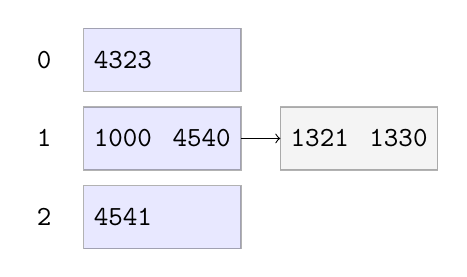
\begin{tikzpicture}
        \foreach \i in {0, 1, 2} {
            \node at (0, 3-\i) {\texttt{\i}};
            
            \draw[fill=blue!30, opacity=0.3] (0.5, \i+1.4) -- (0.5, \i+0.6) -- (2.5, \i+0.6) -- (2.5, \i+1.4) -- cycle;
        };
        \draw[fill=gray!30, opacity=0.3] (3, 2.4) -- (3, 1.6) -- (5, 1.6) -- (5, 2.4) -- cycle;
        
        \node at (1, 1) {\texttt{4541}};
        \node at (1, 2) {\texttt{1000}};
        \node at (2, 2) {\texttt{4540}};
        \node at (1, 3) {\texttt{4323}};
        \node at (3.5, 2) {\texttt{1321}};
        \node at (4.5, 2) {\texttt{1330}};
        
        \draw[->] (2.5, 2) -- (3, 2);
    \end{tikzpicture}
\end{figure}
\noindent The blue blocks are part of the main bucket, while the gray ones are the overflow blocks. We require 4 buckets to hash these values. If we were using heap or sequential representation, we would only need 3 blocks. Since the hashing function does not uniformly distribute the blocks, we instead require 4 here.

Now, we calculate the expected number of block accesses. We are searching with respect to the \texttt{SSN} attribute. We assume that each bucket has equal probability. If the hashed value is 0, then we need to access 1 block and 1 record. The same is true if the hashed value is 2. Instead, if the hashed value is 1, then we need to access 2 blocks- 2 records in the main bucket and 2 overflown buckets. So, the expected block access is
\[\frac{1}{3} \cdot 1 + \frac{1}{3} \cdot 2 + \frac{1}{3} \cdot 1 = \frac{4}{3}.\]
In the best case, we find the value in the first block. So, we would have 1 block access.

If we use the heap file structure, we have 3 blocks. In the worst case, we have 3 block accesses. In the sequential file, we have $\log_2(3) \approx 1.58$ block accesses. In both cases, the best case results in just 1 block access. 

The expected block access for heap representation in the average case is
\[\frac{1 + 3}{2} = 2\]
block accesses. The average block access for hash representation is
\[\frac{1 + 1/2 \cdot 1 + 1/2 \cdot 2 + 1}{3} = 1.15\]
block accesses. For sequential binary search, the average block access is
\[\log_2(3) \approx 1.58\]
block access. So, in all the cases- best, worst and average, the hash representation performs best when checking with respect to the hashed value.

However, range queries are inefficient in hash representation, even when the range is over the hashed field. For each value in the range, we have to find and retrieve the bucket and select the value from the record. The hash function uniformly distributes the values, so we would not want it to be possible to retrieve all values within the same bucket. So, it takes $O(m) + O(mn)$ bucket accesses where $m$ is the range of the distinct values in the range and $O(n)$ overflow blocks per bucket. This is not efficient. Sequential files are much better in this case.

The distribution of values influences the expected cost. This implies that the expected cost is unpredictable to compute in practice. For instance, assume that we have an age distribution as shown in the table below.
\begin{table}[H]
    \centering
    \begin{tabular}{|c|c|}
        \hline
        Age & Count \\
        \hline
        20 & 2 000 \\
        30 & 900 \\
        40 & 800 \\
        50 & 80 \\
        60 & 23 \\
        70 & 80 \\
        \hline
    \end{tabular}
\end{table}
\noindent Moreover, let $\textit{bfr} = 40$ employees per block. For people aged 20, we need to retrieve
\[\operatorname{ceil}(2000/40) = 50\]
blocks. Instead, if we want to get people aged 60, we need to only retrieve
\[\operatorname{ceil}(23/40) = 1\]
block. So, the number of block accesses depends on the value.

Now, assume that we have hash, heap and sorted file like in the example above:
\begin{itemize}
    \item we have 3 blocks in heap and sorted file;
    \item we have 4 blocks in the hash file- 3 main blocks and 1 overflown block.
\end{itemize}
Also, let $k$ be the hash attribute, and let $p\%$ be the proportion of the queries that involve the attribute $k$. Then, in the worst case, heap file would take 3 block accesses- the attribute $k$ does not matter because the search is always linear. Instead, if we use sorted representation, we have
\[p \cdot (\log_2 3) + (1 - p) \cdot 3 = 3 + p \cdot (\log_2 3 - 3).\]
If we have the attribute $k$ in the search, we only require $O(\log_2 b)$ block accesses, but if $k$ is not part of the search, we require $O(b)$ block accesses. Now, if we use hash representation, we have
\[p \cdot (\tfrac{1}{3} \cdot 1 + \tfrac{1}{3} \cdot 2 + \tfrac{1}{3} \cdot 1) + (1 - p) \cdot 3 = 4 - \tfrac{8}{3} p\]
block accesses. We can plot these lines and see which option is better depending on the value of $p$.
\begin{figure}[H]
    \centering
    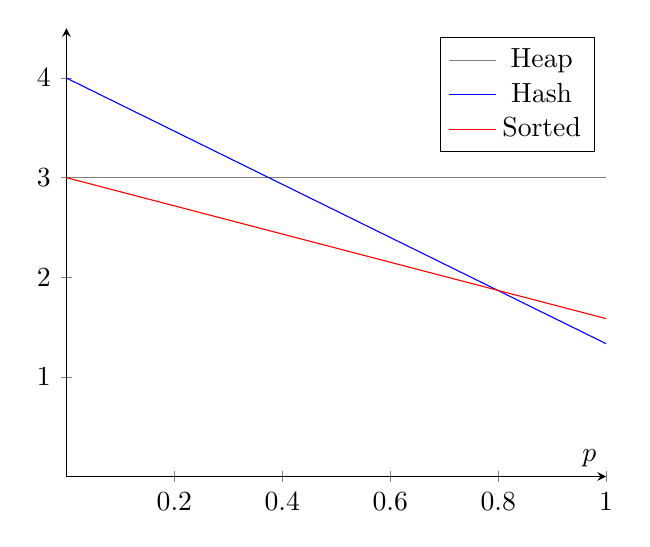
\begin{tikzpicture}
        \begin{axis}[
            axis lines=center,
            xlabel=$p$,
            xmin=0, ymin=0, ymax=4.5,
        ]
            \addplot[
                domain=0:1,
                samples=100,
                gray
            ] {3};
            \addplot[
                domain=0:1,
                samples=100,
                blue
            ] {4 - 8/3*x};
            \addplot[
                domain=0:1,
                samples=100,
                red
            ] {3 + (ln(3)/ln(2) - 3)*x};
            \legend{Heap, Hash, Sorted}
        \end{axis}
    \end{tikzpicture}
\end{figure}
\noindent So, if $p < 0.8$, we should use the sorted representation. Instead, if $p > 0.8$, we should use the hash representation.

\newpage

\section{Indexing Methodology}
We have looked at physical design of the database. The objective there was that, given a specific file type, we provide a primary access path based on a specific searching field. Now, we will look at index design. In this case, our objective is, given any file type, we provide a secondary access path using more than one searching field. 

Adding a secondary access path means that we need to store additional (metadata) files on the disk. Moreover, we need to maintain them so that they are consistent with the actual data. However, we significantly improve the searching process by avoiding linear scanning.

% The image below summarises the trade-off between the overhead (storage and maintenance) and the speed of query execution using primary and second access paths.
% \begin{figure}[H]
%     \centering
%     \begin{tikzpicture}
%         \begin{axis}[
%             axis lines=center,
%             xticklabels={},
%             yticklabels={},
%             xlabel={Overhead},
%             ylabel={Delay},
%             x label style={anchor=north},
%             y label style={anchor=east},
%             xmin=0, xmax=5,
%         ]
%             \addplot[
%             domain=0.5:4.5,
%             samples=100
%             ]{e^(5-x)};
            
%             \draw[fill=red] (0.65, 80) circle (2pt);
%             \node[text width=2cm, align=center] at (1.5, 80) {Primary \\ access paths};
            
%             \draw[fill=blue] (3, 7.5) circle (2pt);
%             \node[text width=2cm, align=center] at (3.2, 20) {Secondary access paths};
%         \end{axis}
%     \end{tikzpicture}
%     \caption{The overhead and the speed of query execution using primary and secondary access paths.}
% \end{figure}
% \noindent We expect that as we increase the storage/maintenance, the time it takes to execute a query decreases exponentially.

When we create an index, we need to follow some principles.
\begin{itemize}
    \item We create one index over one field. This is called the index field. We will only consider indices built on one attribute.
    \item An index is another separate file. This is a metadata file, and is the reason the overhead increases.
    \item All index entries are unique and sorted with respect to the index field. We expect a tuple in the relation to be of the form (\texttt{index-value}, \texttt{block-pointer}).
    The block pointer is the location of the block that contains the entry with the given value.
    \item First, we search within the index file to find the block pointer, and then we access the data block from the data file.
\end{itemize}

For indexing to be more efficient than linear searching, we require the index files to occupy less blocks than the data file. This is true because the index entries are quite small, with only two attributes. So, we can fit in more index entries in a block than data records, i.e. most of the time,
\[\textit{bfr}(\textit{index-file}) > \textit{bfr}(\textit{data-file}).\]

There are 2 indexing strategies. A dense index has an index entry for every record in the file, as illustrated below.
\begin{figure}[H]
    \centering
    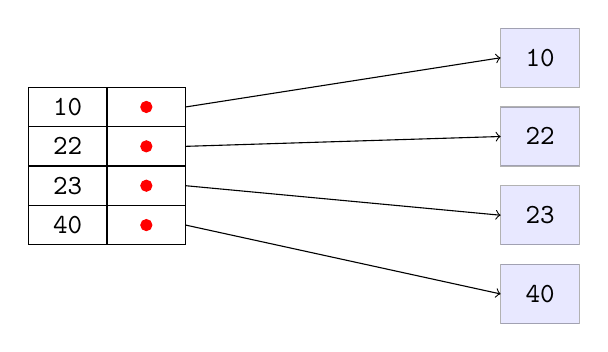
\begin{tikzpicture}
        \draw (2, -2) -- (2, 0)
            -- (0, 0)
            -- (0, -2)
            -- cycle;
            
        \foreach \x[count=\i] in {10, 22, 23, 40} {
            \node at (0.5, -0.5*\i+0.25) {\texttt{\x}};
            \draw (0, -0.5*\i) -- (2, -0.5*\i);
            \draw (1, -0.5*\i) -- (1, -0.5*\i+0.5);
            \filldraw[red] (1.5, -0.5*\i+0.25) circle (2pt);
            
            \draw[fill=blue!30, opacity=0.3] (6, 1-\i) -- (7, 1-\i)
                -- (7, 1-\i+.75)
                -- (6, 1-\i+.75)
                -- cycle;
            
            \node at (6.5, -\i+1.375) {\texttt{\x}};
            
            \draw[->] (2, -0.5*\i+0.25) -- (6, 1-\i+.375);
        }
    \end{tikzpicture}
    \caption{A dense index}
\end{figure}
\noindent So, the index file has the same number of entries as the data file. A sparse index has an index entry for only some of the records, as illustrated below.
\begin{figure}[H]
    \centering
    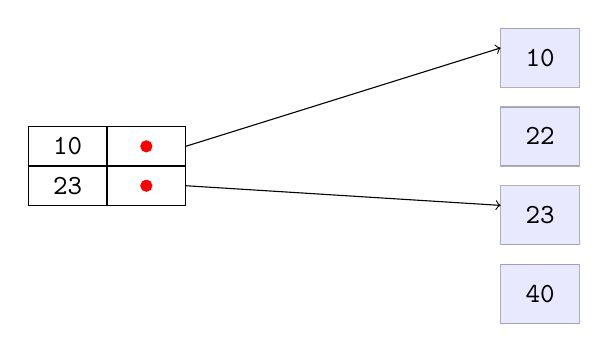
\begin{tikzpicture}
        \draw (2, -1) -- (2, 0)
            -- (0, 0)
            -- (0, -1)
            -- cycle;
            
        \foreach \x[count=\i] in {10, 23} {
            \node at (0.5, -0.5*\i+0.25) {\texttt{\x}};
            \draw (0, -0.5*\i) -- (2, -0.5*\i);
            \draw (1, -0.5*\i) -- (1, -0.5*\i+0.5);
            \filldraw[red] (1.5, -0.5*\i+0.25) circle (2pt);
            
            \draw[->] (2, -0.5*\i+0.25) -- (6, 2.5-\i*2+.5);
        }
            
        \foreach \x[count=\i] in {10, 22, 23, 40} {
            \draw[fill=blue!30, opacity=0.3] (6, 1.5-\i) -- (7, 1.5-\i)
                -- (7, 1.5-\i+.75)
                -- (6, 1.5-\i+.75)
                -- cycle;
            
            \node at (6.5, .5-\i+1.375) {\texttt{\x}};
        }
    \end{tikzpicture}
    \caption{A sparse index}
\end{figure}
\noindent This can be used when the indexing field is how the data files are sorted. So, if the value is 22, we look at the block containing 10- the next block starts with 23, so if 22 is present in the data file, it must lie within this block.

Another expectation we have is than searching over index is faster than over the file. Since indexing file is an ordered file, we can adopt a binary/tree-based approach to find the pointer to the actual data block. This makes the procedure much faster than linear search.

There are 3 types of index types- primary, clustering and secondary index. Primary index is where the index field is an ordering, key field of a sequential file (e.g. \texttt{SSN}, where the file is sorted by \texttt{SSN}). Clustering index is where the index field is an ordering, non-key field of a sequential file (e.g. \texttt{DNO}, where the file is sorted by \texttt{DNO}). Secondary index, where the index field is non-ordering, i.e. the files are not sorted with respect to this attribute. The index field may be key or non-key.

\subsection{Primary Index}
A primary index is built over a sequential file, where the indexing field is the field the files are sorted by. Since the data file is sorted, we can use sparse indexing to index the data files, as illustrated below.
\begin{figure}[H]
    \centering
    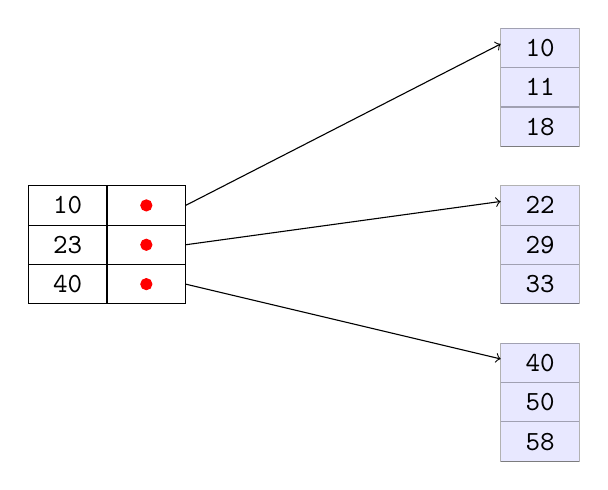
\begin{tikzpicture}
        \draw (2, -1.5) -- (2, 0)
            -- (0, 0)
            -- (0, -1.5)
            -- cycle;
            
        \foreach \x[count=\i] in {10, 23, 40} {
            \node at (0.5, -0.5*\i+0.25) {\texttt{\x}};
            \draw (0, -0.5*\i) -- (2, -0.5*\i);
            \draw (1, -0.5*\i) -- (1, -0.5*\i+0.5);
            \filldraw[red] (1.5, -0.5*\i+0.25) circle (2pt);
            
            \draw[->] (2, -0.5*\i+0.25) -- (6, 3.3-\i*2+.5);
        }
            
        \foreach \i in {0, -1, -2} {
            \draw[fill=blue!30, opacity=0.3] (6, 2*\i+.5) -- (7, 2*\i+.5)
                -- (7, 2*\i+2)
                -- (6, 2*\i+2)
                -- cycle;
        }
                
        \foreach \x[count=\i] in {10, 11, 18} {
            \node at (6.5, 3-\i*.5-.75) {\texttt{\x}};
            \draw[fill=blue!30, opacity=0.3] (6, \i*.5) -- (7, \i*.5);
        }
                        
        \foreach \x[count=\i] in {22, 29, 33} {
            \node at (6.5, 1-\i*.5-.75) {\texttt{\x}};
            \draw[fill=blue!30, opacity=0.3] (6, \i*.5-2) -- (7, \i*.5-2);
        }
                        
        \foreach \x[count=\i] in {40, 50, 58} {
            \node at (6.5, -1-\i*.5-.75) {\texttt{\x}};
            \draw[fill=blue!30, opacity=0.3] (6, \i*.5-4) -- (7, \i*.5-4);
        }
    \end{tikzpicture}
    \caption{Primary Indexing}
\end{figure}
\noindent So, we have one entry in the index file per data block. The $i$-th index entry $(k_i, p_i)$ refers to the $i$-th data block. The value $k_i$ is the field value of the first record in block $i$. The first data-record in block $i$ with value $k_i$ is called the anchor of block $i$.

To find a particular tuple based on the index entry, we first search in the index file the block where we expect this entry to be. The index entries are sorted, so we use a binary search. This gives us the anchor entry of the block. We then load this block and search within the block for the tuple.

If the anchor record is deleted/updated, we need to update the sequential data file- this is a very costly computation. Moreover, after the update, we need to propagate the update to the index file. The index file is also a sequential file, so this too is a costly computation.

If a non-anchor record is updated, we need to update the sequential data file. This need not be propagated to the index file if the order of the blocks isn't affected. If the order of the blocks is affected, or the non-anchor record is deleted, we need to update the data file and the index file like we did previously.

Next, we consider an example. Assume we have the \texttt{EMPLOYEE} table with key attribute \texttt{SSN}.
\begin{itemize}
    \item We have $r = 300 \ 000$ records.
    \item A record takes $R = 100$ bytes.
    \item The block size is $B = 4 \ 096$ bytes.
    \item The attribute \texttt{SSN} occupies 9 bytes.
    \item A pointer occupies 6 bytes.
    \item The data files are sorted with respect to \texttt{SSN}.
\end{itemize}
We want to execute the query
\begin{lstlisting}[language=SQL]
SELECT  *
FROM    EMPLOYEE
WHERE   SSN = k;
\end{lstlisting}
The blocking factor is
\[\textit{bfr} = \operatorname{floor}(B/R) = \operatorname{floor}(4096/100) = 40.\]
So, the number of blocks we need is
\[b = \operatorname{ceil}(r/\textit{bfr}) = 7 \ 500.\]
If we use the primary access path to search for the tuple, a linear search takes on average
\[b/2 = 3 \ 750\]
block accesses, and a binary search takes on average
\[\log_2 b \approx 11.9\]
block accesses. 

We can create a primary index on \texttt{SSN}. In SQL, we do this as follows:
\begin{lstlisting}[language=SQL]
CREATE  INDEX
ON      EMPLOYEE(SSN);
\end{lstlisting}
The index entry has components: $\texttt{(SSN, Pointer)}$. We know that we need 9 bytes for SSN and 6 for the pointer, so we need 15 bytes for each index. Therefore, the indexing blocking factor is
\[\textit{ibfr} = \operatorname{floor}(4096/15) = 273.\]
We have 7 500 data blocks, so 7 500 index tuples. So, we need
\[\textit{ib} = \operatorname{ceil}(7500/273) = 28\]
blocks to store all the index files. So, we require 28 more blocks for primary indices. This is about 0.37\% increase in storage.

Next, we compute the number of block accesses with the primary index. We first search for the SSN in the index, so on average, it takes about
\[\log_2 28 \approx 4.8\]
block accesses to find it. After finding the index block, we need to load the data block. So, we have 6 block accesses to find the relevant tuple. This is a 53\% increase in execution compared to no indexing in the case of a binary search, and 99\% over the linear search. 
% This can be visualised in the graph below.
% \begin{figure}[H]
%     \centering
%     \begin{tikzpicture}
%         \begin{axis}[
%             axis lines=center,
%             xticklabels={},
%             yticklabels={},
%             xlabel={Overhead},
%             ylabel={Delay},
%             x label style={anchor=north},
%             y label style={anchor=east},
%             xmin=0, xmax=5,
%             ymax=95,
%         ]
%             \addplot[
%             domain=0.5:4.5,
%             samples=100
%             ]{e^(5-x)};
            
%             \draw[fill=red] (.5, 90) circle (2pt);
%             \node[text width=2cm, align=center] at (1, 80) {Heap \\ File};
            
%             \draw[fill=red] (1.6, 31) circle (2pt);
%             \node[text width=2cm, align=center] at (2, 38) {Sequential File};
            
%             \draw[fill=blue] (3, 7) circle (2pt);
%             \node[text width=2cm, align=center] at (3.2, 18) {Primary Index};
%         \end{axis}
%     \end{tikzpicture}
%     \caption{Trade off between heap file, sequential file and primary index design in terms of storage and maintenance overhead and search delay.}
% \end{figure}

\subsection{Clustering index}
A clustering index is used to index a sequential file on an ordering, non-key field. The indexing file is a set of cluster of blocks, with a cluster per distinct value. The block pointer points at the first block of the cluster. The other blocks of the same cluster are contiguous and accessed via chain pointers. The clustering index is sparse because we are only using some of the index entries to index the entire data file.

An illustration of clustering index is given below.
\begin{figure}[H]
    \centering
    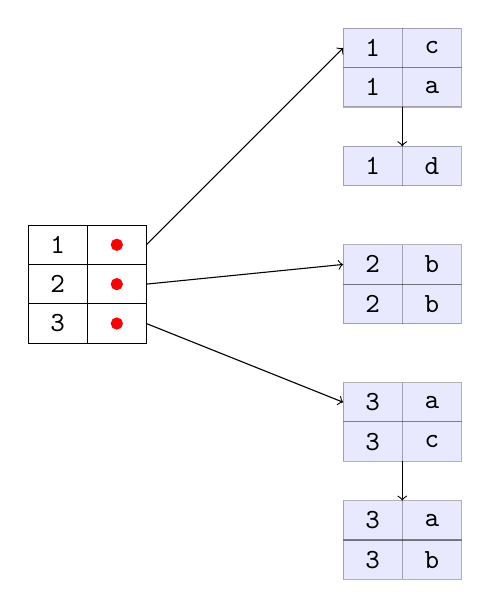
\begin{tikzpicture}
        \draw (0, 0) -- (0, 1.5)
            -- (1.5, 1.5)
            -- (1.5, 0)
            -- cycle;
        
        \foreach \x[count=\i] in {3, 2, 1} {
            \draw (0, \i*0.5-0.5) -- (1.5, \i*0.5-0.5);
            \draw (0.75, \i*0.5-0.5) -- (0.75, \i*0.5);
            
            \node at (0.375, \i*0.5-0.25) {\texttt{\x}};
            \filldraw[red] (1.125, \i*0.5-0.25) circle (2pt);
        }
        
        \draw[->] (1.5, 1.25) -- (4, 3.75);
        
        \foreach \x[count=\i] in {a, c} {
            \draw[fill=blue!30, opacity=0.3] (4, 0.5*\i+3) -- (5.5, 0.5*\i+3)
                -- (5.5, 0.5*\i+2.5)
                -- (4, 0.5*\i+2.5)
                -- cycle;
            
            \draw[fill=blue!30, opacity=0.3] (4.75, 0.5*\i+3) -- (4.75, 0.5*\i+2.5);
            
            \node at (4.375, 0.5*\i+2+0.75) {\texttt{1}};
            \node at (5.125, 0.5*\i+2+0.75) {\texttt{\x}};
        }
        
        \draw[->] (4.75, 3) -- (4.75, 2.5);
        
        \foreach \x[count=\i] in {d} {
            \draw[fill=blue!30, opacity=0.3] (4, 0.5*\i+1.5) -- (5.5, 0.5*\i+1.5)
                -- (5.5, 0.5*\i+2)
                -- (4, 0.5*\i+2)
                -- cycle;
                
            \draw[fill=blue!30, opacity=0.3] (4.75, 0.5*\i+2) -- (4.75, 0.5*\i+1.5);
            
            \node at (4.375, 0.5*\i+1+0.75) {\texttt{1}};
            \node at (5.125, 0.5*\i+1+0.75) {\texttt{\x}};
        }
        
        \draw[->] (1.5, 0.75) -- (4, 1);
            
        \foreach \x[count=\i] in {b, b} {
            \draw[fill=blue!30, opacity=0.3] (4, 0.5*\i-0.25) -- (5.5, 0.5*\i-0.25)
                -- (5.5, 0.5*\i+0.25)
                -- (4, 0.5*\i+0.25)
                -- cycle;

            \draw[fill=blue!30, opacity=0.3] (4.75, 0.5*\i+0.25) -- (4.75, 0.5*\i-0.25);
            
            \node at (4.375, 0.5*\i+0.75-0.75) {\texttt{2}};
            \node at (5.125, 0.5*\i+0.75-0.75) {\texttt{\x}};
        }
        
        \draw[->] (1.5, 0.25) -- (4, -0.75);
        
        \foreach \x[count=\i] in {c, a} {
            \draw[fill=blue!30, opacity=0.3] (4, 0.5*\i-1.5) -- (5.5, 0.5*\i-1.5)
                -- (5.5, 0.5*\i-2)
                -- (4, 0.5*\i-2)
                -- cycle;
            
            \draw[fill=blue!30, opacity=0.3] (4.75, 0.5*\i-1.5) -- (4.75, 0.5*\i-2);
            
            \node at (4.375, 0.5*\i-1-0.75) {\texttt{3}};
            \node at (5.125, 0.5*\i-1-0.75) {\texttt{\x}};
        }
        
        \draw[->] (4.75, -1.5) -- (4.75, -2);
        
        \foreach \x[count=\i] in {b, a} {
            \draw[fill=blue!30, opacity=0.3] (4, 0.5*\i-3) -- (5.5, 0.5*\i-3)
                -- (5.5, 0.5*\i-3.5)
                -- (4, 0.5*\i-3.5)
                -- cycle;
            
            \draw[fill=blue!30, opacity=0.3] (4.75, 0.5*\i-3) -- (4.75, 0.5*\i-3.5);
            
            \node at (4.375, 0.5*\i-2.5-0.75) {\texttt{3}};
            \node at (5.125, 0.5*\i-2.5-0.75) {\texttt{\x}};
        }
    \end{tikzpicture}
    \caption{Clustering Index}
\end{figure}
\noindent The number of index entries is the same as the number of the clusters. Each pointer in the index entry points to the first entry of the cluster. Each block is pointing to the next contiguous blocks using a linked list data structure.

We will now analyse the performance of the clustering index. Assume we have the \texttt{EMPLOYEE} table with non-key attribute \texttt{DNO}.
\begin{itemize}
    \item We have $r = 300 \ 000$ records.
    \item A record takes $R = 100$ bytes.
    \item The block size is $B = 4 \ 096$ bytes.
    \item The attribute \texttt{DNO} occupies 9 bytes.
    \item A pointer occupies 6 bytes.
    \item The data files are sorted with respect to \texttt{DNO}.
    \item There are 10 departments.
    \item The \texttt{DNO} values are uniformly distributed over the tuples, i.e. there are $30 \ 000$ employees in each department.
\end{itemize}
We want to execute the query
\begin{lstlisting}[language=SQL]
SELECT  *
FROM    EMPLOYEE
WHERE   DNO = x;
\end{lstlisting}
The blocking factor is
\[\textit{bfr} = \operatorname{floor}(4096/100) = 40.\]
So, the number of blocks we need is
\[b = \operatorname{ceil}(r/\textit{bfr}) = 7 \ 500.\]

We first consider a linear scan with an exiting feature- we stop as soon as we have found all the tuples. Based on the uniformity assumption, each department has 750 blocks. If we have \texttt{DNO = 1}, then we retrieve the first 750 blocks and then stop. If \texttt{DNO = 2}, then we retrieve the first two 750 blocks and then stop. Assuming that it is equally likely for the \texttt{DNO} to take all these values and that the value \texttt{x} is a valid \texttt{DNO}, the expected block accesses is:
\[\frac{1}{10} \cdot 750 + \frac{1}{10} (750 \cdot 2) + \dots + \frac{1}{10} (750 \cdot 10) = 4125.\]
In general, if we have $n$ clusters and $b$ blocks, then linear search with an exiting feature on an ordered data file is
\[\frac{b(n+1)}{2n}.\]

We can also create a clustering index on DNO. The indexing blocking factor is
\[\textit{ibfr} = \operatorname{floor}(4096/15) = 273.\]
We have 10 data blocks, so we need
\[\textit{ib} = \operatorname{ceil}(10/273) = 1\]
block to store all the index files. So, the overhead is 0.01\% additional storage. When executing the query, we find the block pointer corresponding to \texttt{DNO = x} in 1 block access. Then, we load the 750 contiguous blocks to find all the relevant tuples. This requires 751 block accesses.

We should create a clustering index if it allows us to find the result in fewer block accesses. In particular, if we have $m$ clustering index blocks, $b$ data blocks and $n$ clusters, we should create the index if
\[\log_2 m <  \frac{b(n-1)}{2n} \implies m < 2^{\frac{b(n-1)}{2n}.}\]
% Moreover, as $n \to \infty$, the linear search over an ordering non-key field with exiting feature is bound by $b/2$. So, as 
% i.e. we have an infinite number of distinct values, then the linear search over an ordering non-key field with exiting feature is bound by $b/2$, which is half of the naive linear search, i.e.
% \[\lim_{n \to \infty} \frac{b(n+1)}{2n} = \frac{b}{2} < b.\]

% In the trade-off curve, sequential file and clustering index lie as shown below.
% \begin{figure}[H]
%     \centering
%     \includegraphics[scale=0.5]{src/2.2/2.2.8.PNG}
%     \caption{Trade off between sequential file and clustering index.}
% \end{figure}
% By just storing one extra block, we have an 81.8\% speed up.

\subsection{Secondary Index}
Now, we want to index a file on a non-ordering field. The file might be undordered, hashed, or ordered, but not ordered with respect to the indexing field. There are 2 cases here, where the secondary index is unique or not.

If we want a secondary index on a non-ordering, key field, we need one index entry per data record, i.e. a dense index. This is because the entries are scattered around the data file with respect to this index, and so we cannot use anchors.

An illustration of secondary non-ordering key index is given below:
\begin{figure}[H]
    \centering
    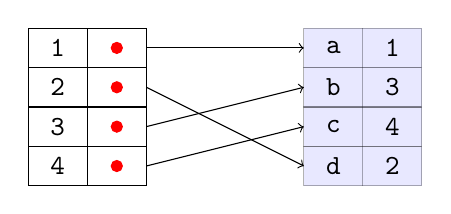
\begin{tikzpicture}
        \draw (1.5, 0.5) -- (3, 0.5)
            -- (3, -1.5)
            -- (1.5, -1.5)
            -- cycle;
        \foreach \x/\y in {-1/4, -0.5/3, 0/2, 0.5/1} {
            \draw (1.5, \x) -- (3, \x);
            \draw (2.25, \x) -- (2.25, \x-0.5);
            
            \node at (1.875, \x-0.25) {\texttt{\y}};
            \filldraw[red] (2.625, \x-0.25) circle (2pt);
        }
        
        \draw[->] (3, 0.25) -- (5, 0.25);
        \draw[->] (3, -0.25) -- (5, -1.25);
        \draw[->] (3, -0.75) -- (5, -0.25);
        \draw[->] (3, -1.25) -- (5, -0.75);
        
        \foreach \x/\y[count=\i] in {d/2, c/4, b/3, a/1} {
            \draw[fill=blue!30, opacity=0.3] (5, \i*0.5-2) -- (6.5, \i*0.5-2)
                -- (6.5, \i*0.5-1.5)
                -- (5, \i*0.5-1.5)
                -- cycle;
            \draw[fill=blue!30, opacity=0.3] (5.75, \i*0.5-1.5-0.5) -- (5.75, \i*0.5-1.5);
            
            \node at (5.375, \i*0.5-1.5-0.25) {\texttt{\x}};
            \node at (6.125, \i*0.5-1.5-0.25) {\texttt{\y}};
        }
    \end{tikzpicture}
    \caption{Secondary Index on a non-ordering, key index}
\end{figure}
\noindent For each index entry, we store the block pointer where the tuple can be found.

Now, we will compute block accesses for a secondary index on a non-ordering key attribute. Assume we have the \texttt{EMPLOYEE} table with non-ordering key attribute \texttt{SSN}. 
\begin{itemize}
    \item We have $r = 300 \ 000$ records.
    \item A record takes $R = 100$ bytes.
    \item The block size is $B = 4 \ 096$ bytes.
    \item The attribute \texttt{SSN} occupies 9 bytes.
    \item A pointer occupies 6 bytes.
\end{itemize}
We want to run the query
\begin{lstlisting}[language=SQL]
SELECT  *
FROM    EMPLOYEE
WHERE   SSN = x;
\end{lstlisting}
The blocking factor is
\[\textit{bfr} = \operatorname{floor}(B/R) = 40\]
records per block. So, we need
\[b = \operatorname{ceil}(r/\textit{bfr}) = 7500\]
blocks to store all the data.

An index entry takes 15 bytes. So, the index blocking factor is
\[\textit{ibfr} = \operatorname{floor}(4096/15) = 273.\]
Since we are using a dense index, we have 300 000 index entries. So, we need
\[\textit{ib} = \operatorname{ceil}(300000/273) = 1099\]
blocks. We have 14\% overhead in that case.

To search for a single employee, we first search within the index. Since the index file is sorted, we can find it in
\[\operatorname{ceil}(\log_2(\textit{ib})) = 11\]
block accesses. Next, we load the unique block pointed by the index entry. So, we require 12 block accesses to find the relevant tuple. If we were to just use a serial search on the file, it would take on average 
\[b/2 = 3750\]
block accesses. So, we have a 99.7\% speed up. 
% This is illustrated below.
% \begin{figure}[H]
%     \centering
%     \includegraphics[scale=0.5]{src/2.2/2.2.11.PNG}
%     \caption{Trade off between heap file and secondary index}
% \end{figure}

The second type of secondary index is on a non-ordering, non-key field. So, some records are having the same indexing value. Moreover, the data files are not sorted with respect to the index attribute. So, we need to store all the block pointers for a given index in yet another file. 

This is illustrated in the figure below.
\begin{figure}[H]
    \centering
    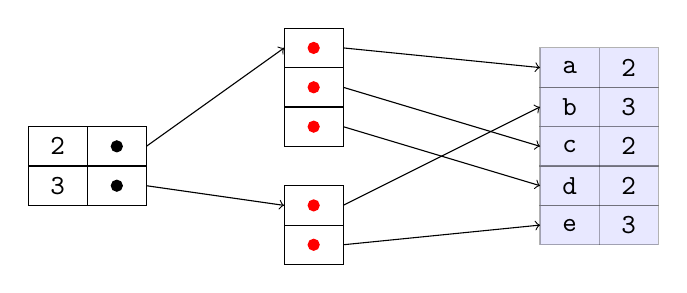
\begin{tikzpicture}
        \draw (-1.5, 0) -- (-1.5, -1)
            -- (0, -1)
            -- (0, 0)
            -- cycle;
        \draw (-0.75, 0) -- (-0.75, -1);
        \draw (-1.5, -.5) -- (0, -.5);
        
        \filldraw[black] (-0.375, -0.25) circle (2pt);
        \filldraw[black] (-0.375, -0.75) circle (2pt);
        \node at (-1.125, -0.25) {\texttt{2}};
        \node at (-1.125, -0.75) {\texttt{3}};
        
        \draw[->] (0, -0.25) -- (1.75, 1);
        \draw[->] (0, -0.75) -- (1.75, -1);
        
        \draw (1.75, 1.25) -- (2.5, 1.25)
            -- (2.5, -0.25)
            -- (1.75, -0.25)
            -- cycle;
        \draw (1.75, -1.75) -- (2.5, -1.75)
            -- (2.5, -0.75)
            -- (1.75, -0.75)
            -- cycle;
        \foreach \i in {0.25, 0.75, 1.25, -0.75, -1.25} {
            \draw (1.75, \i) -- (2.5, \i);
            \filldraw[red] (2.125, \i-0.25) circle (2pt);
        }
        
        \draw[->] (2.5, 1) -- (5, 0.75);
        \draw[->] (2.5, 0.5) -- (5, -0.25);
        \draw[->] (2.5, 0) -- (5, -0.75);
        \draw[->] (2.5, -1) -- (5, 0.25);
        \draw[->] (2.5, -1.5) -- (5, -1.25);
        
        \foreach \x/\y[count=\i] in {e/3, d/2, c/2, b/3, a/2} {
            \draw[fill=blue!30, opacity=0.3] (5, \i*0.5-2) -- (6.5, \i*0.5-2)
                -- (6.5, \i*0.5-1.5)
                -- (5, \i*0.5-1.5)
                -- cycle;
            \draw[fill=blue!30, opacity=0.3] (5.75, \i*0.5-1.5-0.5) -- (5.75, \i*0.5-1.5);
            
            \node at (5.375, \i*0.5-1.5-0.25) {\texttt{\x}};
            \node at (6.125, \i*0.5-1.5-0.25) {\texttt{\y}};
        }
    \end{tikzpicture}
    \caption{Secondary index on a non-ordering, non-key attribute.}
\end{figure}
\noindent In the figure above, we have 2 possible values for the index- \texttt{2} and \texttt{3}. Within the indexing file, we point to a secondary indexing file. In the secondary index file, we have block pointers for all the data records that have the matching index value (a cluster/group). Indexing at the first level is sparse since there are many tuples in the data field with the index value since this value is not unique.

So, there are 2 levels of indirection here. At the first level, we have a block of block pointers of a cluster. At the second level, a block pointer points to the data block that has records within this distinct index value.

% Assume we have the \texttt{EMPLOYEE} table with non-ordering, non-key attribute \texttt{DNO}, where there 
% \begin{itemize}
%     \item We have $r = 300 \ 000$ records.
%     \item A record takes $R = 100$ bytes.
%     \item The block size is $B = 4 \ 096$ bytes.
%     \item The attribute \texttt{DNO} occupies 9 bytes.
%     \item A pointer occupies 6 bytes.
%     \item There are 4 blocks of pointers satisfying \texttt{DNO = 3}.
% \end{itemize}
% We want to execute the query
% \begin{lstlisting}[language=SQL]

% \end{lstlisting}
% In the example above, assume we are searching for \texttt{DNO = 3}. We can use binary search in level 2. There is only one block at level 1 corresponding to \texttt{DNO = 3}, so we can use that to load all the 4 blocks that have \texttt{DNO = 3}. If we do not have this index, we need to linearly scan all the blocks since it is not a unique value. So, we need to access all 7500 blocks. So, using secondary indexing, we have 99.9\% speed up.

\subsection{Multi-level index}
All the index files (primary, clustering and secondary) can be used to build multi-level index files. They are all ordered with respect to the indexing field. Moreover, the indexing field have unique values, and each index entry is of fixed length. This means we can create an primary index on each of these index files. We could even build an index over that index, and so on. This is multi-level indexing.

The original index file is called the base or Level-1 index file. Indexing this index file gives us a Level-2 index file. We can continue this on to get a Level-$t$ index file for any positive integer $t$. Now, we aim to find the best level-$t$ of a multi-level index to expedite the search process trading off speed-up with overhead.

The following is an example of a level-2 index.
\begin{figure}[H]
    \centering
    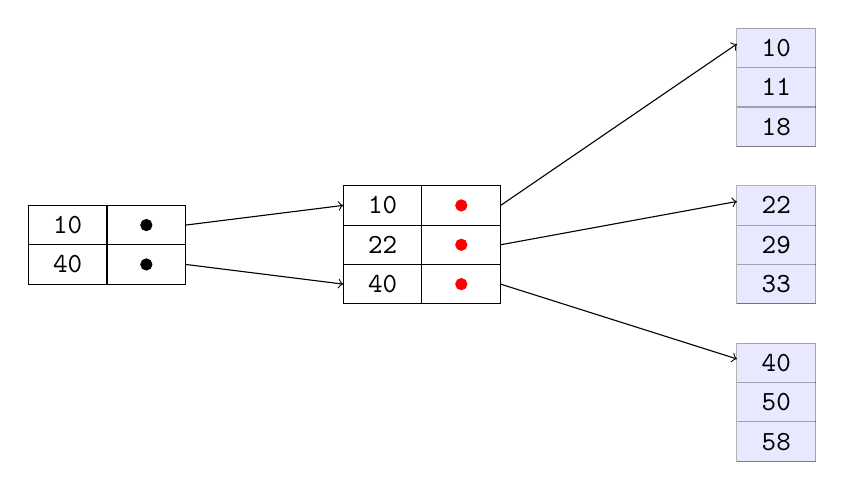
\begin{tikzpicture}
        \draw (-1, -1.25) -- (-1, -0.25)
            -- (-3, -0.25)
            -- (-3, -1.25)
            -- cycle;
        
        \foreach \x[count=\i] in {10, 40} {
            \node at (-2.5, -0.25-0.5*\i+0.25) {\texttt{\x}};
            \draw (-1, -0.25-0.5*\i) -- (-3, -0.25-0.5*\i);
            \draw (-2, -0.25-0.5*\i) -- (-2, -0.25-0.5*\i+0.5);
            \draw[fill=black] (-1.5, -0.25-0.5*\i+0.25) circle (2pt);
            
            \draw[->] (-1, -0.5*\i) -- (1, 0.5-\i+0.25);
        }
            
        \draw (3, -1.5) -- (3, 0)
            -- (1, 0)
            -- (1, -1.5)
            -- cycle;
            
        \foreach \x[count=\i] in {10, 22, 40} {
            \node at (1.5, -0.5*\i+0.25) {\texttt{\x}};
            \draw (1, -0.5*\i) -- (3, -0.5*\i);
            \draw (2, -0.5*\i) -- (2, -0.5*\i+0.5);
            \filldraw[red] (2.5, -0.5*\i+0.25) circle (2pt);
            
            \draw[->] (3, -0.5*\i+0.25) -- (6, 3.3-\i*2+.5);
        }
            
        \foreach \i in {0, -1, -2} {
            \draw[fill=blue!30, opacity=0.3] (6, 2*\i+.5) -- (7, 2*\i+.5)
                -- (7, 2*\i+2)
                -- (6, 2*\i+2)
                -- cycle;
        }
                
        \foreach \x[count=\i] in {10, 11, 18} {
            \node at (6.5, 3-\i*.5-.75) {\texttt{\x}};
            \draw[fill=blue!30, opacity=0.3] (6, \i*.5) -- (7, \i*.5);
        }
                        
        \foreach \x[count=\i] in {22, 29, 33} {
            \node at (6.5, 1-\i*.5-.75) {\texttt{\x}};
            \draw[fill=blue!30, opacity=0.3] (6, \i*.5-2) -- (7, \i*.5-2);
        }
                        
        \foreach \x[count=\i] in {40, 50, 58} {
            \node at (6.5, -1-\i*.5-.75) {\texttt{\x}};
            \draw[fill=blue!30, opacity=0.3] (6, \i*.5-4) -- (7, \i*.5-4);
        }
    \end{tikzpicture}
    \caption{A 2-level index}
\end{figure}
\noindent The first index is a primary index, so it is using anchors. Also, the second level is a primary index, so it points to the anchors within the level-1 index file. The level-2 index has 1 block (containing 2 records), so we should not create level-3 index on it.

In general, we should stop not create level-$t+1$ index if level-$t$ where the top-level index has 1 block. So, given a level-1 index with blocking factor $m$ entries/block, the multi-level index is of maximum level
\[t = \log_m b.\]
The value $m$ is known as fan-out. 

% We can plot the search time for different complexities as the number of block accesses increases.
% \begin{figure}[H]
%     \centering
%     \includegraphics[scale=0.5]{src/2.2/2.2.15.PNG}
%     \caption{How the number of block accesses affects search time of the algorithm}
% \end{figure}
% \noindent As the base increases, the search process is almost independent of the number of blocks. This means that the design is scalable; it does not depend on the data size.

% We will illustrate how multi-level index files can be used to get a specific file.
% \begin{figure}[H]
%     \centering
%     \includegraphics[scale=0.5]{src/2.2/2.2.16.PNG}
%     \caption{A multi-level index}
% \end{figure}
\noindent If we want to find a tuple from a level-$t$ index, we first load the $t$-level index block. Using this block, we can load a single $t-1$-level block, and so on. We continue this until we load a L1 block. So, we need precisely $t$ block accesses to load the L1 data block. Finally, we load the actual data file block using the L1 index. If it takes $n$ block accesses to retrieve the data block from the L1 block, it will take us
\[t + n = \log_m b + n\]
block accesses to retrieve the relevant tuple(s).

Now, assume that we have the \texttt{EMPLOYEE} table on the non-ordering key attribute \texttt{SSN}. We have $b = 7 \ 500$ blocks and $r = 300 \ 000$ records. Previously, we saw that the blocking factor of the L1 index is $m = 273$. At L1 index, we have 
\[b_1 = \operatorname{ceil}(r/m) = 1 \ 099\]
index blocks, since the index is dense. So, in level-2, we have $1 \ 099$ index entries, and we require
\[b_2 = \operatorname{ceil}(b_1/m) = 5\]
blocks to store them. Furthermore, at level-3, we have $5$ index entries, and we just require
\[b_3 = \operatorname{ceil}(b_2/m) = 1\]
block for it. Since we just need 1 block here, we build a 3-level index. Now, to find the unique employee we are searching for, we just need 4 block accesses- 3 going from one index level to a lower level, and the last one to get the data block. At level-1, we required 12 block accesses. Moreover, we need on average 3 750 block accesses with a linear search.

% We can plot the performance of heap file, L1 and L3 indices in the trade off curve below.
% \begin{figure}[H]
%     \centering
%     \includegraphics[scale=0.5]{src/2.2/2.2.17.PNG}
%     \caption{Trade off between overhead and speed between heap file, L1 secondary index and L3 secondary index.}
% \end{figure}
\newpage

\section{B and B+ Trees}
For multi-level indices, we search for a record over a $t$-level index with $t+1$ block accesses. However, insertions, deletions and updates over the data file are reflected over the multi-level indices. This makes the operations costly. This is because all encapsulated indexes are physically ordered files. So, all updates should be reflected to all levels.

We will try to define a dynamic multi-level indices. This means that the data structure should:
\begin{itemize}
    \item adjust to deletions and insertions of records;
    \item expand and shrink following the distribution of the index values; and
    \item be self-balancing (subtrees should be of the same depth).
\end{itemize}
We will do this using B and B+ Trees.

We can envisage a multi-level index as a tree. This can be done by turning it clockwise by 90 degrees. For example, consider the following diagram.
\begin{figure}[H]
    \centering
    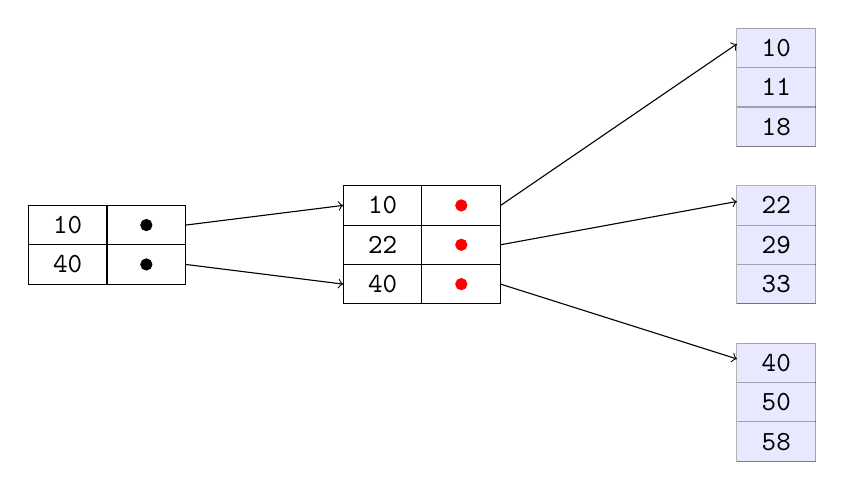
\begin{tikzpicture}
        \draw (-1, -1.25) -- (-1, -0.25)
            -- (-3, -0.25)
            -- (-3, -1.25)
            -- cycle;
        
        \foreach \x[count=\i] in {10, 40} {
            \node at (-2.5, -0.25-0.5*\i+0.25) {\texttt{\x}};
            \draw (-1, -0.25-0.5*\i) -- (-3, -0.25-0.5*\i);
            \draw (-2, -0.25-0.5*\i) -- (-2, -0.25-0.5*\i+0.5);
            \draw[fill=black] (-1.5, -0.25-0.5*\i+0.25) circle (2pt);
            
            \draw[->] (-1, -0.5*\i) -- (1, 0.5-\i+0.25);
        }
            
        \draw (3, -1.5) -- (3, 0)
            -- (1, 0)
            -- (1, -1.5)
            -- cycle;
            
        \foreach \x[count=\i] in {10, 22, 40} {
            \node at (1.5, -0.5*\i+0.25) {\texttt{\x}};
            \draw (1, -0.5*\i) -- (3, -0.5*\i);
            \draw (2, -0.5*\i) -- (2, -0.5*\i+0.5);
            \filldraw[red] (2.5, -0.5*\i+0.25) circle (2pt);
            
            \draw[->] (3, -0.5*\i+0.25) -- (6, 3.3-\i*2+.5);
        }
            
        \foreach \i in {0, -1, -2} {
            \draw[fill=blue!30, opacity=0.3] (6, 2*\i+.5) -- (7, 2*\i+.5)
                -- (7, 2*\i+2)
                -- (6, 2*\i+2)
                -- cycle;
        }
                
        \foreach \x[count=\i] in {10, 11, 18} {
            \node at (6.5, 3-\i*.5-.75) {\texttt{\x}};
            \draw[fill=blue!30, opacity=0.3] (6, \i*.5) -- (7, \i*.5);
        }
                        
        \foreach \x[count=\i] in {22, 29, 33} {
            \node at (6.5, 1-\i*.5-.75) {\texttt{\x}};
            \draw[fill=blue!30, opacity=0.3] (6, \i*.5-2) -- (7, \i*.5-2);
        }
                        
        \foreach \x[count=\i] in {40, 50, 58} {
            \node at (6.5, -1-\i*.5-.75) {\texttt{\x}};
            \draw[fill=blue!30, opacity=0.3] (6, \i*.5-4) -- (7, \i*.5-4);
        }
    \end{tikzpicture}
\end{figure}
\noindent We can rotate it clockwise by 90 degrees to get the following tree.
\begin{figure}[H]
    \centering
    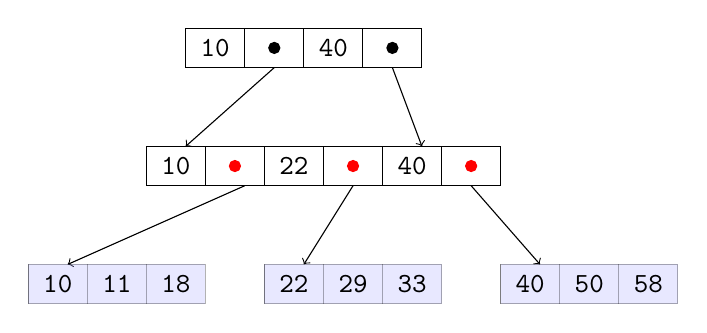
\begin{tikzpicture}
        \draw (0, 0) -- (3, 0)
            -- (3, 0.5)
            -- (0, 0.5)
            -- cycle;
        
        \foreach \x[count=\i] in {10, 40} {
            \node at (\i*0.75*2-1.125, 0.25)  {\texttt{\x}};
            \draw[fill=black] (\i*0.75*2-0.375, 0.25) circle (2pt);
            \draw (\i*0.75, 0) -- (\i*0.75, 0.5);
            \draw (\i*0.75+1.5, 0) -- (\i*0.75+1.5, 0.5);
        }
        
        \draw[->] (1.125, 0) -- (0, -1);
        \draw[->] (2.625, 0) -- (3, -1);
        
        \draw (0-0.5, 0-1.5) -- (4.5-0.5, 0-1.5)
            -- (4.5-0.5, 0.5-1.5)
            -- (0-0.5, 0.5-1.5)
            -- cycle;
        
        \foreach \x[count=\i] in {10, 22, 40} {
            \node at (\i*0.75*2-1.125-0.5, 0.25-1.5)  {\texttt{\x}};
            \filldraw[red] (\i*0.75*2-0.375-0.5, 0.25-1.5) circle (2pt);
            \draw (\i*0.75-0.5, 0-1.5) -- (\i*0.75-0.5, 0.5-1.5);
            \draw (\i*0.75+1.5-0.5, 0-1.5) -- (\i*0.75+1.5-0.5, 0.5-1.5);
        }
        
        \draw[->] (0.75, -1.5) -- (-1.5, -2.5);
        \draw[->] (2.125, -1.5) -- (1.5, -2.5);
        \draw[->] (3.625, -1.5) -- (4.5, -2.5);
        
        \draw[fill=blue!30, opacity=0.3] (0-2, 0-3) -- (2.25-2, 0-3)
            -- (2.25-2, 0.5-3)
            -- (0-2, 0.5-3)
            -- cycle;
            
        \foreach \x[count=\i] in {10, 11, 18} {
            \node at (\i*0.75-0.375-2, 0.25-3)  {\texttt{\x}};
            \draw[fill=blue!30, opacity=0.3] (\i*0.75-0.75-2, 0-3) -- (\i*0.75-0.75-2, 0.5-3);
        }
        
        \draw[fill=blue!30, opacity=0.3] (0+1, 0-3) -- (2.25+1, 0-3)
            -- (2.25+1, 0.5-3)
            -- (0+1, 0.5-3)
            -- cycle;
            
        \foreach \x[count=\i] in {22, 29, 33} {
            \node at (\i*0.75-0.375+1, 0.25-3)  {\texttt{\x}};
            \draw[fill=blue!30, opacity=0.3] (\i*0.75-0.75+1, 0-3) -- (\i*0.75-0.75+1, 0.5-3);
        }
        
        \draw[fill=blue!30, opacity=0.3] (0+4, 0-3) -- (2.25+4, 0-3)
            -- (2.25+4, 0.5-3)
            -- (0+4, 0.5-3)
            -- cycle;
            
        \foreach \x[count=\i] in {40, 50, 58} {
            \node at (\i*0.75-0.375+4, 0.25-3)  {\texttt{\x}};
            \draw[fill=blue!30, opacity=0.3] (\i*0.75-0.75+4, 0-3) -- (\i*0.75-0.75+4, 0.5-3);
        }
    \end{tikzpicture}
\end{figure}
\noindent Here, the root is the level-2 index. The children of the root are level-1 index blocks. The leaves are the actual data blocks.

There is a limitation to this. The tree need to be balanced. This is because it does not adjust to keys' distribution. That is, the leaf nodes are at different levels. The number of block accesses in a multi-level index depends on the depth of the tree, so we would like the tree to be as balanced as possible. In the worst case, we have a linked list of nodes.

Our first challenge is to ensure that the tree is balanced by minimising the tree depth $t$. This challenge has two parts- how do we deal with insertion into a full node, and deletion of a node. We can split a node into two if the node is full, and merge two nodes if a node is to be deleted. This increases the overhead, but is required to keep the tree balanced.

\subsection{B Tree}
B Trees are used for secondary indices with a key, non-ordering attribute. A B tree node of order $p$ splits the searching space up to $p$ subspaces. We assume $p > 2$. A node is of the form
\[\{P_1, (K_1, Q_1), P_2, (K_2, Q_2), \dots, P_{p-1}, (K_{p-1}, Q_{p-1}), P_p\},\]
where 
\begin{itemize}
    \item $K_i$ is a key value, 
    \item $P_i$ is a tree pointer for those tuples with $X < K_i$,
    \item $P_{i+1}$ is a tree pointer for those tuples with $X > K_i$,
    \item $Q_i$ is a block pointer for $K_i$.
\end{itemize}
A pictorial representation of this is given below.
\begin{figure}[H]
    \centering
    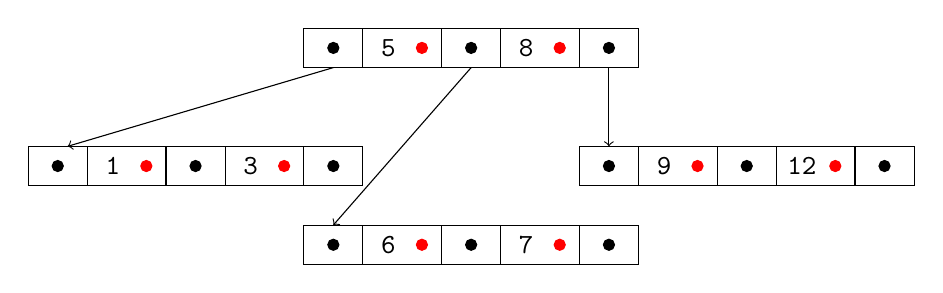
\begin{tikzpicture}
        \bnode{0}{0}{5, 8} 
        \bnode{-3.5}{-1.5}{1, 3} 
        \bnode{0}{-2.5}{6, 7} 
        \bnode{3.5}{-1.5}{9, 12} 
        
        \draw[->] (0.375, 0) -- (-3, -1);
        \draw[->] (2.125, 0) -- (0.375, -2);
        \draw[->] (3.875, 0) -- (3.875, -1);
    \end{tikzpicture}
\end{figure}

The advantage of B trees is that every time we descend a level, we split the searching space into $p$ subtrees, which exponentially lowers the searching space. If $p = 2$, this is equivalent to binary search. We typically have $p > 2$. Like in the case above, a tree of order $p$ can store up to $p$ tree pointers (shown in black) and up to $p-1$ key values and their block pointers (shown in red).

When searching for a tuple of a value using a B tree, we start from the root and descend in the right branches until we get to a key value corresponding to the tuple. Then, we access the corresponding data block and return the matching tuple. 

Normally, a data block contains all the elements of the tree. So, each tree node corresponds to a block. We now consider the number of block accesses we need to find the right tuple with the B tree given above:
\begin{itemize}
    \item If we search for 8, we first access the root block. Since this node contains the value 8, we can access the data block containing 8 with another block access. In total, we need 2 block accesses.
    \item If we search for 7, we first access the root block. This node does not contain 7, so we descend the middle branch. This block does contain the value 7, so we can access the data block containing 7 with another block access. In total, we need 3 block accesses.
    \item If we search for 31, we first access the root block. This node does not contain 7, so we descend the root branch. This block also doesn't contain 31, but we know there is no right tree pointer here. This means that there is no record corresponding to the value 31. So, we just need 2 block accesses.
\end{itemize}

Now, assume that we have created a 3-level B tree of order $p = 23$ that is $69\%$ full. So, in each block, we store
\[69\% \times 23 \approx 16\]
tree pointers, and 15 data pointers. In that case, the root block contains 16 tree pointers and 15 data pointers. At level 1, we have 16 blocks, each of which contains 16 tree pointers and 15 data pointers. At level 2, we have $16^2$ blocks, each of which contains 16 tree pointers and 15 data pointers. At level 3, we have $16^3$ blocks, each of which contains no tree pointers and 15 data pointers. This is summarised in the table below.
\begin{table}[H]
    \centering
    \begin{tabular}{|c|c|c|}
        \hline
        level & data pointers & tree pointers \\
        \hline
        0 & 15 & 16 \\
        1 & $16 \cdot 15$ & $16^2$ \\
        2 & $16^2 \cdot 15$ & $16^3$ \\
        3 & $16^3 \cdot 15$ & 0 \\
        \hline
    \end{tabular}
\end{table}
In total, we can store 65 535 data pointers and 4 368 tree pointers. If we want to add an extra tuple, then we would need to add another level. Since B trees are balanced, we need to add all $16^4$ tree pointers. But then, 93.3\% of the leaf nodes at level 4 are empty. We need to choose a good value for $p$ to reduce this redundancy. This gives rise to another challenge.

Now, assume that the block size is $B = 512$ bytes, data pointer $Q = 7$ bytes, tree pointer $P = 6$ bytes and key values $V = 9$ bytes. Then, the index is
\[65 \ 536 \cdot (7 + 9) + 4 \ 368 \cdot 6 = 1.02 \text{ MB}.\]
Moreover, each block has size
\[15 \cdot (7 + 9) + 16 \cdot 6 = 336 \text{ bytes}.\]
So, the blocking factor 
\[\textit{bfr} = \operatorname{floor}(512/336) = 1.\]
Finally, the number of blocks we need is
\[1 + 16 + 16^2 + 16^3 = 4369\]
blocks.

\subsection{B+ Trees}
A B Tree gives rise to a big metadata. We need to find another data structure so that it has the advantages of B tree while minimising storage. A B tree node stores a lot of data: tree pointers, data pointers and key values. We need tree pointers and key values to navigate the B tree. 

We want to be storage efficient by freeing up space from the nodes. Also, we want to be search efficient by maximising the fan out (the splitting factor) of a node. We can increase the order of the node to increase fan out. To do this, we get rid of data pointers from the nodes. We still need to store data pointers, but we can remove them from non-leaf nodes.

In a B+ Tree, we have 2 types of nodes. An internal node guides the search process, and only have tree pointers and key values. A leaf node points to actual data blocks. To maximise fan out, internal nodes have no data pointers. However, we need to go to the leaf to access any data pointers. Nonetheless, since we have removed data pointers from the nodes, this process is quite fast. 

Moreover, the leaf nodes hold all the key values sorted and their corresponding data pointers. Also, some key values are replicated in the internal nodes to guide and expedite the search process. This corresponds to medians of key values in sub-trees.

A B+ internal node of order $p$ is of the form
\[\{P_1, K_1, P_2, K_2, \dots, P_{p-1}, K_{p-1}, P_p\},\]
where
\begin{itemize}
    \item $K_i$ is a key value,
    \item $P_i$ is a tree pointer for those tuples with $X < K_i$,
    \item $P_{i+1}$ is a tree pointer for those tuples with $X > K_i$.
\end{itemize}
A pictorial representation of this is given below.
\begin{figure}[H]
    \centering
    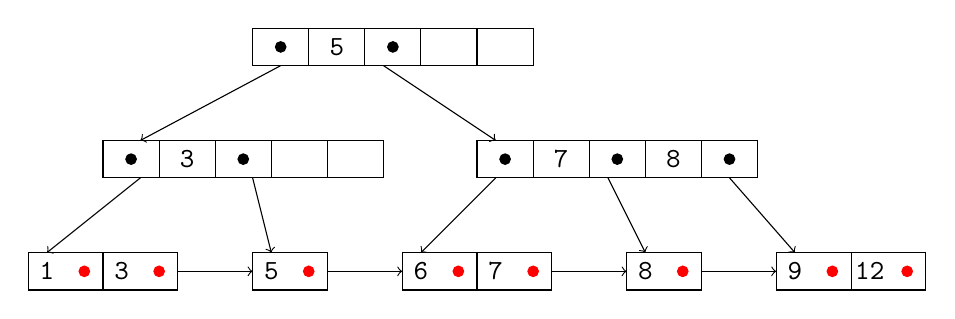
\begin{tikzpicture}[scale=0.95]
        \bplusinternalnodesng{0}{0}{5}
        \bplusinternalnodesng{-2}{-1.5}{3}
        \bplusinternalnodedbl{3}{-1.5}{7, 8}
        \bplusleafnodedbl{-3}{-3}{1, 3}
        \bplusleafnodesng{0}{-3}{5}
        \bplusleafnodedbl{2}{-3}{6, 7}
        \bplusleafnodesng{5}{-3}{8}
        \bplusleafnodedbl{7}{-3}{9, 12}

        \draw[->] (0.375, 0) -- (-1.5, -1);
        \draw[->] (1.75, 0) -- (3.25, -1);

        \draw[->] (-1.5, -1.5) -- (-2.75, -2.5);
        \draw[->] (0, -1.5) -- (0.25, -2.5);
        \draw[->] (3.25, -1.5) -- (2.25, -2.5);
        \draw[->] (4.75, -1.5) -- (5.25, -2.5);
        \draw[->] (6.375, -1.5) -- (7.25, -2.5);
        
        \draw[->] (-1, -2.75) -- (0, -2.75);
        \draw[->] (1, -2.75) -- (2, -2.75);
        \draw[->] (4, -2.75) -- (5, -2.75);
        \draw[->] (6, -2.75) -- (7, -2.75);
    \end{tikzpicture}
\end{figure}
\noindent A B+ tree of order $p$ can store up to $p$ tree pointers and up to $p-1$ key values. 

A B+ internal node of order $p_L$ is of the form
\[\{(K_1, Q_1), (K_2, Q_2), \dots, (K_{p_L}, Q_{p_L}), P_{\text{next}}\},\]
where
\begin{itemize}
    \item $K_i$ is a key value,
    \item $Q_i$ is a data pointer for $K_i$,
    \item $P_{\text{next}}$ points to the next block of leaf nodes.
\end{itemize}
% A pictorial representation of this is given below.
% \begin{figure}[H]
%     \centering
%     \includegraphics[scale=0.45]{src/2.3/2.3.6.PNG}
% \end{figure}
\noindent We have a linked list of leaf nodes. All the leaf nodes are at the same level, meaning that the tree is balanced.

% An example of a B+ tree is given below.
% \begin{figure}[H]
%     \centering
%     \includegraphics[scale=0.5]{src/2.3/2.3.7.PNG}
% \end{figure}
% \noindent Here, the internal nodes have order $p = 3$ and leaf nodes have order $p_L = 2$. 

The leaf nodes are linked and sorted by key. All keys of the file appear at the leaf nodes. The leaf nodes contain data pointers only, to expedite navigation. Leaf nodes are balanced for constant I/O cost. Some selected keys are replicated in the internal nodes for efficiency.

To find the block containing a given value, we must always descend to the leaf nodes. So, it will always take 3 block accesses to find the relevant tuple, assuming it is present.

We will now compare the number of block accesses required when executing the following query for B and B+ trees:
\begin{lstlisting}[language=SQL]
SELECT  * 
FROM    EMPLOYEE
WHERE   SSN >= 3 AND SSN <= 10;
\end{lstlisting}
We have the following B Tree.
\begin{figure}[H]
    \centering
    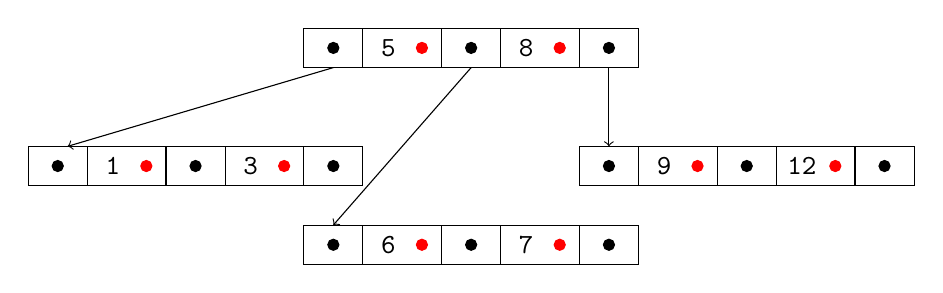
\begin{tikzpicture}
        \bnode{0}{0}{5, 8} 
        \bnode{-3.5}{-1.5}{1, 3} 
        \bnode{0}{-2.5}{6, 7} 
        \bnode{3.5}{-1.5}{9, 12} 
        
        \draw[->] (0.375, 0) -- (-3, -1);
        \draw[->] (2.125, 0) -- (0.375, -2);
        \draw[->] (3.875, 0) -- (3.875, -1);
    \end{tikzpicture}
\end{figure}
\noindent We access the root block and get the values \texttt{SSN = 5} and \texttt{SSN = 8}. Since they are both in the range, we need to access all the 3 branches. 

On the other hand, the B+ Tree we have is the following:
\begin{figure}[H]
    \centering
    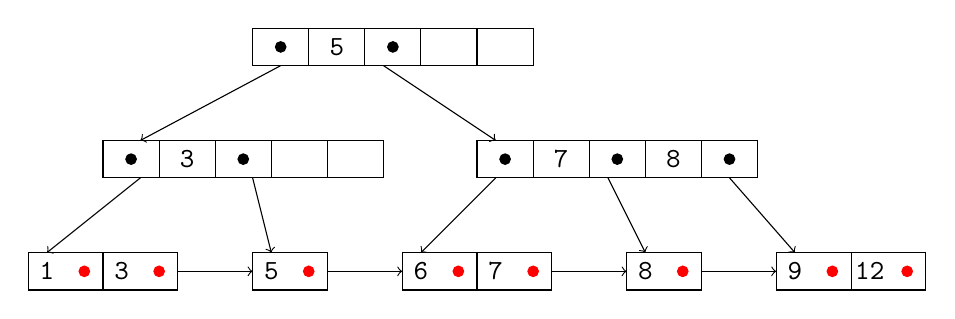
\begin{tikzpicture}[scale=0.95]
        \bplusinternalnodesng{0}{0}{5}
        \bplusinternalnodesng{-2}{-1.5}{3}
        \bplusinternalnodedbl{3}{-1.5}{7, 8}
        \bplusleafnodedbl{-3}{-3}{1, 3}
        \bplusleafnodesng{0}{-3}{5}
        \bplusleafnodedbl{2}{-3}{6, 7}
        \bplusleafnodesng{5}{-3}{8}
        \bplusleafnodedbl{7}{-3}{9, 12}

        \draw[->] (0.375, 0) -- (-1.5, -1);
        \draw[->] (1.75, 0) -- (3.25, -1);

        \draw[->] (-1.5, -1.5) -- (-2.75, -2.5);
        \draw[->] (0, -1.5) -- (0.25, -2.5);
        \draw[->] (3.25, -1.5) -- (2.25, -2.5);
        \draw[->] (4.75, -1.5) -- (5.25, -2.5);
        \draw[->] (6.375, -1.5) -- (7.25, -2.5);
        
        \draw[->] (-1, -2.75) -- (0, -2.75);
        \draw[->] (1, -2.75) -- (2, -2.75);
        \draw[->] (4, -2.75) -- (5, -2.75);
        \draw[->] (6, -2.75) -- (7, -2.75);
    \end{tikzpicture}
\end{figure}
\noindent We access the root block and get the value \texttt{SSN = 5}. We want to find the tuple satisfying \texttt{SSN = 3}, so we just need to take the left branch. Now, we take the left branch in level 1. Then, we have found the first block that we require. We can make use of the sorted structure of the leaf nodes to find all the other tuples that satisfy \texttt{SSN >= 3} and \texttt{SSN <= 10}.

By removing the data pointers from internal nodes, we obtain higher fan out, thus more index entries and quicker search process. We show this with an example. Assume we have block size $B = 512$ bytes, key value $V = 9$ bytes, data pointer $Q = 7$ bytes, tree pointer $P = 6$ bytes. A B tree node will take up
\[p \cdot 6 + (p-1) \cdot (9+7) = 22p - 16\]
bytes. The biggest possible value of $p$ satisfying $22p - 16 \leq 512$ is $p = 24$. On the other hand, for a B+ tree internal node, we require
\[p \cdot 6 + (p-1) \cdot 9 = 15p - 9\]
bytes. Here, the biggest possible value of $p$ is $p = 34$. For a B+ leaf node, we require
\[p_L \cdot (9 + 7) + 9\]
bytes. So, the biggest possible value of $p_L$ is $p_L = 31$. Clearly, we can store more entries in both the B+ tree nodes compared to a B tree. The fan out has indeed increased.

Now, we will construct a 3-level B+ Tree of order $p = 34$ and $p_L = 31$ that is $69\%$ full. So, we can fit 23 tree pointers in an internal node and 21 data pointers in a leaf node. The table below summarises the number of tree pointers and key values we can hold in the first 3 levels.
\begin{table}[H]
    \centering
    \begin{tabular}{|c|c|c|}
        \hline
        level & key values & tree pointers \\
        \hline
        0 & 22 & 23 \\
        1 & $23 \cdot 22$ & $23^2$ \\
        2 & $23^2 \cdot 22$ & $23^3$ \\
        \hline
    \end{tabular}
\end{table}
\noindent So, we can fit 12 720 tree pointers. At level 3, we can fit $23^3 \cdot 21 = 255 \ 507$ key values and data pointers. Moreover, we require
\[1 + 23 + 23^2 + 23^3 = 12 \ 720\]
blocks.

For a B tree, we saw that we can store $65 \ 535$ key values and data pointers in the tree in a very similar scenario. Using a B+ tree, we have almost multiplied the capacity by 4. However, we require about 3 times more blocks for a B tree. Nonetheless, adding a new tuple to the B tree can be costly (e.g. if we add a $65 \ 536$th tuple). This is not the case for B+ trees- we might not even have to add the new entry to an internal block. Moreover, adding to the leaf nodes is simple since it is a linked list, even if we need to keep it sorted.

Next, we compare block accesses and the number of extra blocks required to evaluate a query based on a secondary, non-ordering key field, where:
\begin{itemize}
    \item the size of a block $B = 512$ bytes;
    \item the number of tuples $r = 100 \ 000$;
    \item the blocking factor $\textit{bfr} = 10$ records/block;
    \item a pointer takes up 10 bytes;
    \item the indexing key takes 10 bytes.
\end{itemize}
We will consider 3 ways we can evaluate this query below.
\begin{itemize}
    \item First, we consider a linear search. Since there are 100 000 records and $\textit{bfr} = 10$, we have 10 000 data blocks. On average, the linear search will require 5 000 block accesses.
    
    \item Next, we consider a secondary index. Since the index is secondary, we need a dense index- every data record appears in the index, with a data pointer (10 bytes) and the key value (10 bytes). So, each record takes up 20 bytes. We know a block can store 512 bytes, so each block can hold
    \[\operatorname{floor}(512/20) = 25\]
    tuples. In that case, we require
    \[\operatorname{ceil}(100 \ 000/25) = 4 \ 000\]
    extra blocks to store the secondary index. Moreover, using the secondary index, we require $\log_2 4000 \approx 12$ block accesses to find the right tuple on the secondary index file, and then a further data block access to retrieve the tuple. In total, the search requires 13 block accesses. 
    
    \item Finally, we consider a B+ tree index of order 25. So, each internal node can hold 24 key values and 25 tree pointers, and a leaf block can hold 24 key values and data pointers. A pointer and an indexing key takes 10 bytes, so an internal node takes up
    \[25 \cdot 10 + 24 \cdot 10 = 490\]
    bytes. Moreover, a leaf node takes up
    \[24 \cdot 10 + 24 \cdot 10 + 10 = 490\]
    bytes. So, we can fit 1 internal/leaf node per block. We require a 3-level B+ tree to store all the 100 000 tuples in the leaf node, where the following table shows how many entries are present in the internal nodes.
    \begin{table}[H]
        \centering
        \begin{tabular}{|c|c|c|}
            \hline
            level & key values & tree pointers \\
            \hline
            0 & 24 & 25 \\
            1 & $25 \cdot 24$ & $25^2$ \\
            2 & $25^2 \cdot 24$ & $25^3$ \\
            \hline
        \end{tabular}
    \end{table}
    So, at level 3, we have
    \[25^3 \cdot 24 = 375 \ 000\]
    data pointers/key values. Since we only have $100 \ 000$ tuples, we are only using up about $30\%$ of the leaf nodes. Moreover, we need
    \[1 + 25 + 25^2 + 25^3 = 16 \ 276\]
    extra blocks to store the B+ tree. Nonetheless, we can find a tuple using a B+ tree with just 5 block accesses:
    \begin{enumerate}
        \item we access the root internal node, 
        \item we descend to the relevant level 1 internal node,
        \item we descend to the relevant level 2 internal node,
        \item we descend to the relevant level 3 leaf node, and
        \item we retrieve the relevant data block.
    \end{enumerate}
\end{itemize}

Next, we consider when range queries are better (over a secondary, non-ordering key attribute) executed with a linear search or B+ tree. Assume that we have the query
\begin{lstlisting}[language=SQL]
SELECT  AVG(SALARY) 
FROM    EMPLOYEE 
WHERE   SSN >= L AND SSN <= U;
\end{lstlisting}
Here,
\begin{itemize}
    \item there are $b = 1 \ 250$ blocks,
    \item there are $n = 1 \ 250$ employees,
    \item the blocking factor $\textit{bfr} = 1$ employee/block,
    \item \texttt{SSN} takes up 10 bytes,
    \item a pointer takes up $P = 10$ bytes,
    \item the B+ tree is of order $p = 5$ and $p_L = 10$,
    \item the leaf nodes are full,
    \item the SSN values range from 1 to 1250.
\end{itemize}
We know that an internal node can hold 4 key values and 5 data pointers. So, we need a 3-level B+ tree so that the leaf nodes can hold the $1 \ 250$ records. The table below shows how many entries are present in the internal nodes.
\begin{table}[H]
    \centering
    \begin{tabular}{|c|c|c|}
        \hline
        level & key values & tree pointers \\
        \hline
        0 & 4 & 5 \\
        1 & $5 \cdot 4$ & $5^2$ \\
        2 & $5^2 \cdot 4$ & $5^3$ \\
        \hline
    \end{tabular}
\end{table}
\noindent So, at level 3, we precisely have
\[5^3 \cdot 10 = 1 \ 250\]
key values/data pointers. Let $\alpha = \frac{U - L}{1250}$ be the ratio of employees selected by the query. When we execute this range query over the B+ tree, we need 3 block accesses to descend from the root to the leaf node containing the data pointer for \texttt{SSN = L}. Each leaf node contains 10 blocks, so we approximately need to access 
\[\frac{U - L}{10} = \frac{1250 \alpha}{10} = 125 \alpha\]
leaf blocks. Moreover, we need to access all $U - L = 1250 \alpha$ data blocks. Overall, we need to access
\[3 + 125 \alpha + 1250 \alpha = 3 + 1375 \alpha\]
blocks. Using a linear search, we need to access all the 1250 blocks since the tuples are not sorted with respect to \texttt{SSN}. Therefore, for B+ trees to be useful, we require 
\[3 + 1375 \alpha < 1250 \implies \alpha < \frac{1247}{1375} \approx 0.906.\]
So, if the ratio is less than $90.6\%$, then we should use B+ tree. Otherwise, we should use linear searching. 
% This can be seen in the graph below.
% \begin{figure}[H]
%     \centering
%     % \includegraphics[scale=0.6]{src/2.3/2.3.8.PNG}
%     \begin{tikzpicture}
%         \begin{axis}[
%             axis lines=center,
%             ymax=25, ymin=0,
%             xmin=0, xmax=1,
%             ytick={0.5, 20},
%             yticklabels={3, 1250},
%             xtick={0.75, 1},
%             xticklabels={0.906, 1},
%             ylabel={block access},
%             xlabel={range length}
%         ]
%             \draw (0, 0.5) -- (1, 25);
%             \draw (0, 20) -- (1, 20);
%         \end{axis}
%     \end{tikzpicture}
% \end{figure}


\end{document}
